\chapter{Nutzerstudie}\label{study}

Wie in der Zielsetzung festgelegt, wurde die Usability des digitalen Prototypen für die Erstellung, Bearbeitung und Löschung von Feedback 
in einer Nutzerstudie evaluiert. Da im Prototypen zwei unterschiedliche Darstellungsformen für die Feedbacks implementiert ergaben sich daraus die Aufgaben: Wie konnten die Bearbeitung und Löschung von Feedback gelöst werden und welcher Unterschied in der Usability hinsichtlich der zwei verschiedenen Darstellungsformen festgestellt werden kann.

Im Kapitel \ref{anlayse_capter} Abschnitt \ref{brand_abschnitt} sowie im Abschnitt \ref{ipi_section} wurden Studien betrachtet, welche unterschiedliche Darstellungsformen 
miteinander vergleichen. Auf Grundlage der Ergebnissen, die \citeauthor{Brandenburg2019} in \cite{Brandenburg2019} identifiziert hat - nämlich dass sich die Darstellung als Annotationen am Produkt für Vergleichsaufgaben besser eignet - wurden in dieser Studie zwei gerichtete Hypothesen aufgestellt. 
 
\section{Aufbau der Studie}

\textbf{Versuchspersonen}

An der Studie nahmen 12 Versuchspersonen im Durchschnittsalter von 25 Jahren (Standardabweichung 5,1) teil.  Davon waren vier weiblich und 8 männlich. 
Alle Versuchsteilnehmer waren Studierende. Zehn von ihnen sind im Studiengang Angewandte Informatik, eine Person im Maschinenbau und eine weitere Person in Filmregie immatrikuliert.

Drei der Versuchspersonen haben angegeben regelmäßig Erfahrung mit virtuellen Umgebungen zu haben. Weitere fünf Versuchspersonen haben angegeben, dass sie virtuelle Umgebungen schon 
einmal gesehen oder ausprobiert haben. Nur zwei haben angegeben noch keine Erfahrung bisher zu haben. 
Außerdem haben 8 Versuchspersonen angegeben, dass sie seit mehr als drei Jahren Erfahrung mit Smartphones haben welche mit dem Betriebssystem Android betrieben werden. Zwei haben angegeben keine 
Erfahrung mit Android zu haben. 

Vier der Versuchspersonen gaben an, etwa einmal die Woche Feedback zu Produkten in Online Einkaufsportalen zu lesen. Zwei gaben an, seltener als einmal im Monat Bewertungen zu Produkten zu schreiben und eine Person gab
an, zwei bis drei mal im Monat Bewertungen zu schreiben. 

Elf Versuchspersonen gaben an, dass es ihnen selten bis gelegentlich schwer falle, bestimmte Stellen oder Positionen an einem Produkt zu beschreiben oder Beschreibungen von anderen zu verstehen. Nur ein Teilnehmer gab an, mit 
solchen Beschreibungen keine Schwierigkeiten zu haben. 

\textbf{Material: }

Für den Versuch wurde auf einem Smartphone mit des Typs: \textit{Samsung Galaxy S8} durchgeführt. Auf dem Endgerät war das Betriebssystem Android in der Version 9 installiert. 
Als Produkt wurde das 3D-Modell eines Smart Tripelec genommen. Hierbei handelt es sich um ist ein Fahrrad welches im Sitzen gefahren werden kann. Abbildung \ref{img:trip} zeigt das verwendete Modell.

\begin{figure}[H]
	\centering 
	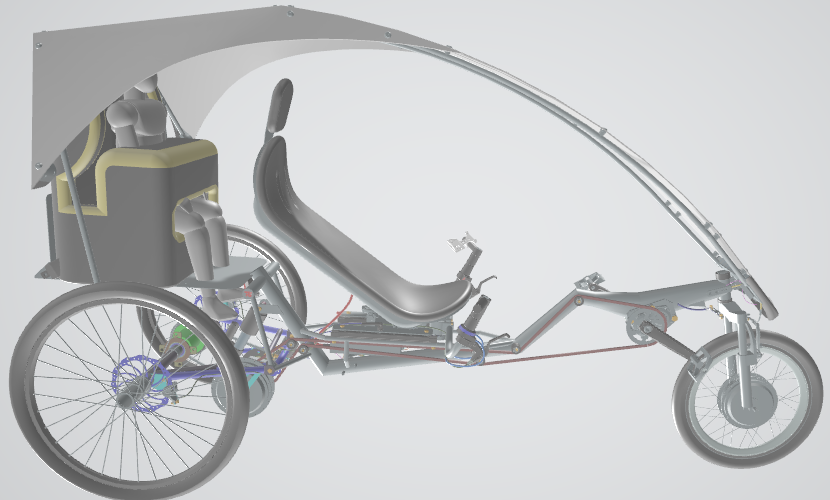
\includegraphics[width=.6\textwidth]{resources/evaluation/SmartTripelec.png}
	\caption{3D Modell Smart Tripelec Quelle: Eigene Abbildung}
	\label{img:trip}
\end{figure}

Leider war es aus organisatorischen Gründen nicht möglich das physische Produkt für die Durchführung der Studie zur Verfügung da zu haben. So wurde der Versuch ohne Überlagerung des realen Produktes auf dem virtuellen Produkt durchgeführt. 

Das Nutzungserleben (engl. User Experience, kurz UX) wurde nach dem meCUE Fragebogen von \citeauthor{Minge2013} operationalisiert. Dieser Fragebogen ist modular aufgebaut und beinhaltet die vier Module der 
Produktwahrnehmung, Emotionen, Konsequenzen und des Gesamturteil. Abbildung \ref{img:mequeMoudul} zeigt den Aufbau dieser Module.

\begin{figure}[H]
	\centering 
	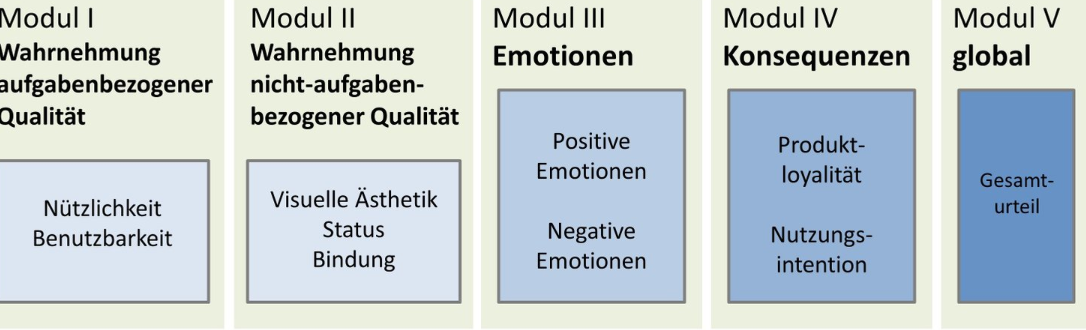
\includegraphics[width=.6\textwidth]{resources/evaluation/meQueModul.png}
	\caption{Module des meQue Fragebogens. Quelle: \cite[S.~4]{Minge2013}}
	\label{img:mequeMoudul}
\end{figure} 

In den Modulen M1 bis M3 werden in diesem Fragebogen Aussagen formuliert, deren Zustimmung über ein Likert skaliertes Antwortformat erfasst werden \footnote{Skalenwert von 1 bis 7: ``lehne völlig ab``, ``lehne ab``, ``lehne eher ab``, ``weder
	noch``, ``stimme eher zu``, ``stimme zu``, ``stimme völlig zu``}\cite{Minge2013}. Im Modul vier kann eine Bewertung von –5 bis 5 (Schrittweite 0,5) als Gesamturteil abgegeben werden. 

\textbf{Unabhängige Variablen:}

Die unabhängige Variable (UV) ist die Darstellungsform des zu bearbeitenden Feedback. Die Darstellungsform des Feedback wird zweifach gestuft in: 

\begin{itemize}
\item Darstellung des Feedback als Annotation auf dem Produkt sowie
\item Darstellung des Feedback als Listenansicht 
\end{itemize}

\textbf{Abhängig Variablen}

Objektiv abhängige Variablen sind die Dauer der Bearbeitung des Feedback (Zeit vom Start der Anwendung bis zur Öffnung des Formulars) für die beiden Darstellungsformen sowie für die Darstellung als Annotation für die andren Aufgaben: Erstellung und Löschung von Feedback. Desweiteren zählen die Werte aus dem meQue Fragebogen zu den abhängen Variablen.

\textbf{Prozedur}

Zunächst haben die Versuchsteilnehmer einen demografischen Fragebogen ausgefüllt. Danach wurde die Studie erläutert und eine Einweisung in die Aufgaben gegeben. 
Dies erfolgte in schriftlicher Form. Die Studien sowie Aufgabenbeschreibungen befinden sich im Anhang. 

Die Aufgaben waren: 

\begin{itemize}
	\item Vier neue Feedback erstellen. Der Inhalt der Feedbacks wurde in der Aufgabenbeschreibung vorgegeben. 
	\item Die zuvor erstellten Feedbacks in der Darstellungsvariante der Annotation bearbeiten. In der Aufgabenbeschreibung wurde vorgegeben, was sich am Feedback ändern sollte.
	\item Die zuvor erstellten Feedbacks in der Darstellungsvariante Liste bearbeiten. In der Aufgabenbeschreibung wurden die durchzuführenden Änderungen vorgegeben.
	\item Die vier Feedback in der Darstellungsvariante der Annotation sollten gelöscht werden.
\end{itemize}

Nach jeder Aufgabenbearbeitung (z. B. nach vier Iterationen zum Erstellen von Feedback) wurde der MeQue Fragebogen von den Teilnehmern ausgefüllt und die jeweils durchgeführte Interaktion bewertet. 

\textbf{Hypothesen}

Auf Grundlage der Analyse 

H1: Die Darstellung der Feedbacks als Annotation erhöhen die Nützlichkeit, Benutzbarkeit und Zufriedenheit.\\
\vspace{2mm}H2: Die Zeit, in das Formular für die Bearbeitung der Feedback zu gelangen, wird mit der Darstellung als Annotation auf dem Produkt weniger Zeit in Anspruch nehmen als mit der Darstellung in Listenansicht. 

Beide Darstellungsformen wurden von den gleichen Versuchspersonen durchgeführt.\\ 
Als Signifikanzniveau wurde ($\alpha$)= 0,05 festgelegt. 

\section{Erhebung}

\textbf{Ergebnisse}

Abbildung \ref{img:avg_meQue_listAnnotation} zeigt die Mittelwerte für die mit dem meQue Fragebogen bewerteten Produkteigenschaften. 
Sie stellt die Bewertung der Produkteigenschaften für die Bearbeitung der Annotation mit der Darstellung als Listenansicht und der Annoation Ansicht nebeneinander. 

\begin{figure}[H]
	\centering
	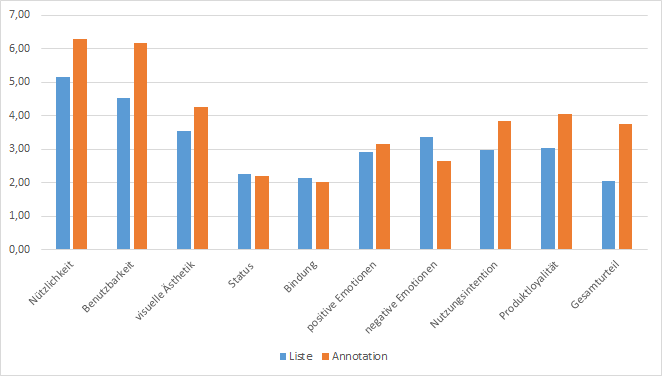
\includegraphics[width=1.0\textwidth]{resources/evaluation/diagrammmittel_vergleich_liste_annotation.png}
	\caption{Vergleich der Mittelwerte aus meQue Fragebogen für Listen vs. Annotation Ansicht \\Quelle:  Eigene Darstellung}
	\label{img:avg_meQue_listAnnotation}
\end{figure}

Auf Abbildung \ref{img:pWerte} sind die p-Werte für Mittelwerte für die Bewertung der Produkteigenschaften zu sehen. Diese wurden in einem T-Test mit ein Signifikanzniveau von Alpha $\alpha$ = 0,05 berechnet. 

\begin{figure}[H]
	\centering
	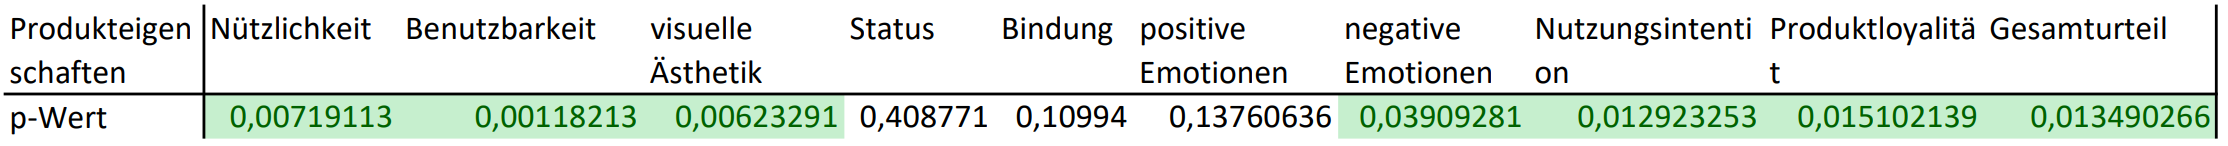
\includegraphics[width=1.0\textwidth]{resources/evaluation/pWerte.png}
	\caption{p-Werte für den Vergleich von meQue Fragebogen Liste vs. Annotation Ansicht\\Quelle:  Eigene Darstellung}
	\label{img:pWerte}
\end{figure}

Abbildung \ref{img:mwListeAnno} zeigt eine Vergleich der Mittelwerte  für die Zeit in Sekunden vom Start der Anwendung bis zur Öffnung des Bearbeitungsformulars für die beiden Darstellungsvarianten Liste und Annotation.  

\begin{figure}[H]
	\centering
	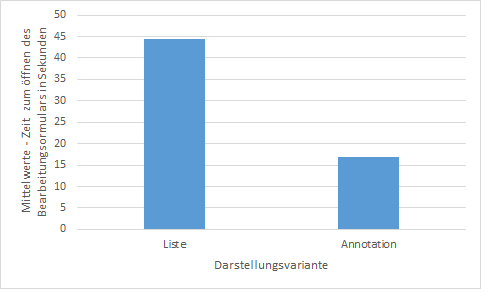
\includegraphics[width=.8\textwidth]{resources/evaluation/mittelwerte_liste_anno.png}
	\caption{Vergleich der Mittelwerte (Liste vs. Annotation) über alle Versuchspersonen und Iterationen. \\Quelle: Eigene Darstellung}
	\label{img:mwListeAnno}
\end{figure}

Hier ergab ein T-Test mit Signifikanzniveau von Alpha $\alpha$ = 0,05 einen p-Wert von 0,064

Auf Abbildung \ref{img:mwUsability} sind die Mittelwerte der aufgabenbezogenen Produktqualitäten der Nützlichkeit (engl. Usability) und Nutzbarkeit (engl. Utility)- bewertet nach dem meQue Fragebogen - für die 
Aufgaben Erstellung, Bearbeitung und Löschung von Feedback zu sehen. Die Abbildung \ref{img:mwTimes} zeigt die durchschnittlichen Zeiten für diese Aktionen.

\begin{figure}[H]
	\centering
	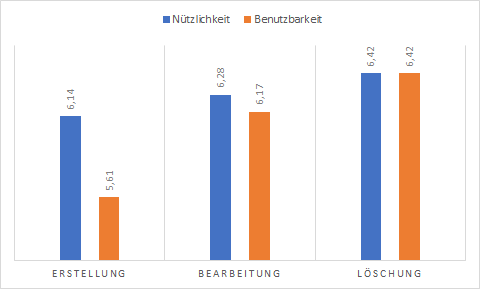
\includegraphics[width=.8\textwidth]{resources/evaluation/MittelWerteUsability.png}
	\caption{Mittelwerte Usability u. Utility für die Aufgaben: Erstellen - Bearbeiten - Löschen in Annotation Ansicht \\Quelle: Eigene Darstellung}
	\label{img:mwUsability}
\end{figure}

\begin{figure}[H]
	\centering
	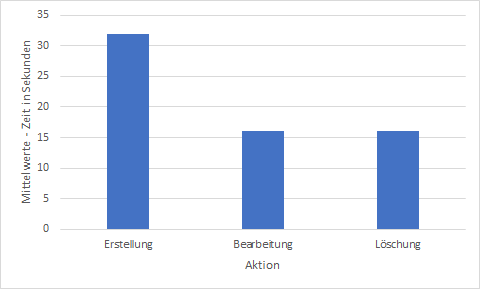
\includegraphics[width=.8\textwidth]{resources/evaluation/mittelwerte_alle_aktionen.png}
	\caption{Mittelwerte der Zeiten für die Aufgaben: Erstellen - Bearbeiten - Löschen in Annotation Ansicht \\Quelle: Eigene Darstellung}
	\label{img:mwTimes}
\end{figure}

\section{Diskussion}

Auf Grundlage der aus der Auswertung der erhobenen Daten gewonnenen Erkenntnisse kann folgendes festgehalten werden:

In Bezug auf die aufgabenbezogenen Qualitäten (wie Gebrauchtstauglich- und Brauchbarkeit) des Prototypen werden das \textit{Relative Pointing} sowie die Darstellung des Feedback als Annotation mit Verbindungslinie zum Produkt, bevorzugt. Sowohl die Mittelwerte des me-Que Fragebogen, in welcher die Aufgaben Bearbeiten und Löschen mit über 6 und die Aufgabe Erstellen mit über 5,5 bei einer Bewertungsskala bis 7 bewertet wurden, als auch die gemessenen Zeiten für diese Aufgabenbearbeitung bestätigen dies: Der Mittelwert für die Erstellung eines Feedback beträgt 30 Sekunden, für die Aufgaben Bearbeiten und Löschen sind es 16 Sekunden.

Die Hypothese H1, kann auf Grundlage der berechneten p-Werte für die Produkteigenschaften Nützlichkeit, Nutzbarkeit, visuelle Ästhetik, negative Emotionen, Nutzungsintention sowie Gesamturteil bestätigt werden.
Hypothese H2 jedoch kann mit einem ermittelten p-Wert von 0,064 nicht bestätigt werden, da dieser Wert über dem festgelegten Signifikanzniveau von 0,05 liegt

Insgesamt kann zusammenfassend gesagt werden, dass die Ansicht mit Annotationen für die Aufgaben ein Feedback auf dem Produkt zu bearbeiten oder zu löschen gegenüber der Listenansicht bevorzugt werden kann. 
Der Prototyp zeigt eine hohe Usability, hat jedoch nach den Ergebnissen des meQue Fragebogens zu urteilen hinsichtlich der Produkteigenschaften \textit{visuelle Ästhetik}, \textit{positive Emotionen}, \textit{Status}, \textit{Nutzungsintention} sowie \textit{Gesamturteil} deutliches Verbesserungspotenzial.
 
